\chapter{Anforderungen}\index{Anforderungen}\label{chp:Anforderungen}
In der Softwareentwicklung erl�utern Anforderungen alle Funktionen eines Softwareprojekts, die ein Auftraggeber vom fertigen Produkt erwartet. Spezifiziert werden die Anforderungen im Lastenheft, welches direkt vom Auftraggeber an den Auftragnehmer verteilt wird.\\
Die Anforderungen werden f�r gew�hnlich in die zwei Kategorien funktional und nichtfunktional unterteilt. 
\begin{quote}
\textbf{Funktionale Anforderungen} \textit{beschreiben die Merkmale einer Funktion, also was das Produkt tun soll.}\\
\textbf{Nichtfunktionale Anforderungen} \textit{beschreiben die Eigenschaften des Produktes, also we das Produkt etwas tun soll.}
\end{quote}
Als Beispiel nehmen wir wieder unser bekanntes Blackboard, welches wir bereits detailiert in den Kapiteln \ref{ssec:UseCases} \nameref{ssec:UseCases} sowie \ref{ssec:Mockups} \nameref{ssec:Mockups} besprochen haben. Bei unserem Blackboard haben wir die drei funktionalen Anforderungen \textit{Notiz hinzuf�gen}, \textit{Notiz bearbeiten}, \textit{Notiz l�schen} und die eine nichtfunktionale Anforderung \textit{Desgin}. Betrachten wir uns die funktionale Anforderung \textit{Notiz hinzuf�gen} in Abb. \ref{fig:LastenheftAnforderungF1}.
\begin{figure}[H]
\centering
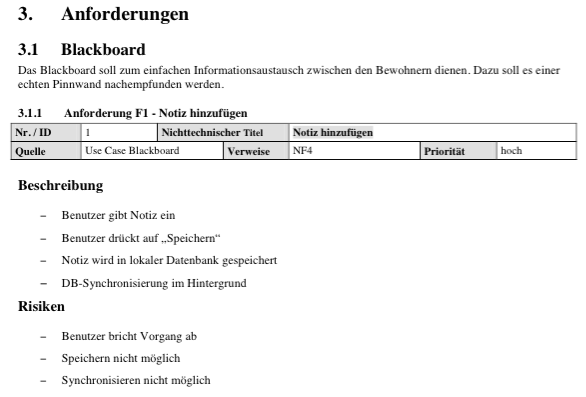
\includegraphics[width=\linewidth]{images/vorgehensweise/lastenheft/LastenheftAnforderungenBlackBoard.png}
\caption{Anforderung F1 - Notiz hinzuf�gen (Blackboard)}
\label{fig:LastenheftAnforderungF1}
\end{figure}
Zu Beginn wird die Eigenschaft jeder Anforderung in ein bis zwei kurzen S�tzen erl�utert. Daraufhin folgt eine Tabelle mit charakteristischen Merkmalen der Anforderung. Jeder Anforderung wird eine eindeutige, fortlaufende  ID zugeteilt. Au�erdem wird ein nichttechnischer Titel vergeben. Als Quelle der Anforderung dient ein anderes Dokument der Projektarbeit, im besten Fall bereits verf�gbar und f�r alle abrufbar. Meistens wird ein Dokument aus den Mockups oder Use-Cases als Quelle herangezogen. Die Verweise geben alle weiterf�hrenden Dokumente an, in denen die Anforderung weiter ausgef�hrt wird oder welche, die auf die Zusammenarbeit mit dieser Anforderung unverzichtbar sind. Letztendliche kann noch eine Priorit�t vergeben werden. Wir haben uns, mit Ausnahmen, bei vielen unserer funktionalen Anforderungen f�r eine hohe Priorit�t und bei vielen nichtfunktionalen Anforderungen f�r eine normale Priorit�t entschieden.\\
Nach der Tabelle folgt eine stichwortartige Beschreibung des grunds�tzlich vorgesehenen Ablaufes. Hierbei wird dargestellt, wie das System sowie der Benutzer agieren muss und welche Konsequenz zu erwarten sind.
Zuletzt werden alle bekannten Risiken aufgez�hlt und stichwortartig beschrieben.\\
\\

\section{Anforderungen f�r DorMApp}\label{AnforderungenDorMApp}
Alle funktionalen Anforderungen werden als \textit{Anforderung F\#} und alle nichtfunktionalen Anforderungen werden als \textit{Anforderung NF\#} gekennzeichnet.\\
Es folgen nun alle Anforderung f�r unsere App, sortiert nach den Hauptfunktionen.\\
\begin{itemize}
	\item \textbf{Blackboard}
		\begin{itemize}
			\item \textit{Anforderung F1 - Notiz hinzuf�gen}
			\item \textit{Anforderung F2 - Notiz bearbeiten}
			\item \textit{Anforderung F3 - Notiz l�schen}
			\item \textit{Anforderung NF4 - Design}			
		\end{itemize}
\end{itemize}

\begin{itemize}
	\item \textbf{Putzplan}
		\begin{itemize}
			\item \textit{Anforderung F5 - Aufgabe erledigen}
			\item \textit{Anforderung NF6 - Design}
		\end{itemize}
\end{itemize}

\begin{itemize}
	\item \textbf{Einkaufsliste}
		\begin{itemize}
			\item \textit{Anforderung F7 - Artikel hinzuf�gen}
			\item \textit{Anforderung F8 - Artikel l�schen}
			\item \textit{Anforderung F9 - Artikel gekauft}
			\item \textit{Anforderung NF10 - Design}
		\end{itemize}
\end{itemize}

\begin{itemize}
	\item \textbf{Kalender}
		\begin{itemize}
			\item \textit{Anforderung F11 - Kalendereintrag eintragen}
			\item \textit{Anforderung F12 - Kalendereintrag bearbeiten}
			\item \textit{Anforderung F13 - Kalendereintrag l�schen}
			\item \textit{Anforderung NF14 - Design}
		\end{itemize}
\end{itemize}

\begin{itemize}
	\item \textbf{Web Login}
		\begin{itemize}
			\item \textit{Anforderung F15 - Web Login}
			\item \textit{Anforderung F16 - Eingabekontrolle}
			\item \textit{Anforderung F17 - Passwort vergessen}
			\item \textit{Anforderung NF18 - Design}
		\end{itemize}
\end{itemize}

\begin{itemize}
	\item \textbf{Web Oberfl�che}
		\begin{itemize}
			\item \textit{Anforderung F19 - Benutzerverwaltung}
			\item \textit{Anforderung F20 - Terminkalenderverwaltung}
			\item \textit{Anforderung F21 - Putzplanverwaltung}
			\item \textit{Anforderung F22 - Systemeinstellungen}
			\item \textit{Anforderung NF23 - Design}
		\end{itemize}
\end{itemize}